\documentclass{standalone}% For the example only, any class will do

\usepackage{tikz}
\usetikzlibrary{positioning}% To get more advances positioning options
\usetikzlibrary{arrows}% To get more arrow heads

\begin{document}
\beginpgfgraphicnamed{survey-f1}
        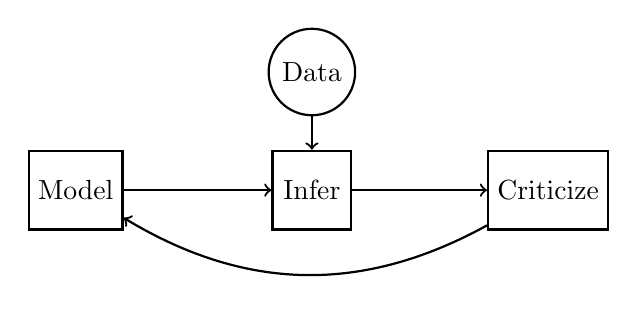
\begin{tikzpicture}
          [
          Box/.style={rectangle, draw=black!, fill=green!0, thick, minimum size=10mm},
          Gray/.style={rectangle, draw=black!, fill=gray!35, thick, minimum size=1mm},
          Round/.style={circle, draw=black!, fill=green!0, thick, minimum size=1mm},
          ]
          % Nodes
          \node[Round] (Data) at(0, 1.5) {Data};
          \node[Box] (Model) at(-3, 0) {Model};
          \node[Box] (Infer) at(0, 0) {Infer};
          \node[Box] (Crit) at (3, 0) {Criticize};

          % Lines
          \path [->, draw, thick] (Model) -- (Infer);
          \path [->, draw, thick] (Infer) -- (Crit);
          \path [->, draw, thick] (Crit) edge[bend left] (Model);
          \path [->, draw, thick] (Data) -- (Infer);

          % 

        \end{tikzpicture}
\endpgfgraphicnamed
\end{document}
%%% Local Variables:
%%% mode: latex
%%% TeX-master: t
%%% End:
